\documentclass[12pt]{report} % You can use 'article' or 'book' class as well

\usepackage{graphicx} % For including images
\usepackage{amsmath}
\usepackage{amssymb}
\usepackage{pgfplots}

\begin{document}

% Title page
\begin{titlepage}
	\centering
	\vspace*{1cm} % Adjusts vertical space for the image
	% Insert your image (use the actual path and filename of your image)
	\includegraphics[width=0.3\textwidth]{../images/KMITL Logo.png} % Adjust width as needed

	\vspace{1cm} % Vertical space after the image
	{\LARGE \textbf{Week 5 Homework}} \\[0.5cm] % Title
	\vspace{0.5cm}
	{\large \textbf{Probability Model and Data Analysis}} \\[0.5cm]
    {\large \textbf{Software Engineering Program,}} \\[0.5cm]
	{\large \textbf{Department of Computer Engineering,}} \\[0.5cm]
	{\large \textbf{School of Engineering, KMITL}} \\[1cm]
	{\Large 67011352 Theepakorn Phayonrat}[0.5cm] % Authors (Use \\ the separate authors)
\end{titlepage}

\section*{Homework of PMF and CDF of Discrete Random Variables}

\subsection*{Question 1}

\noindent For random variables X and R defined in Example 2.5, \\
1. Find the following probabilities: \\
\noindent (a) $P[X = 0]$ \\
(b) $P[X < 3]$ \\
(c) $P[R > 0]$ \\

\subsection*{Answer}

\noindent (a) $P[X = 0] = \frac{1}{8}$ \\
(b) $P[X < 3] = \frac{7}{8}$ \\
(c) $P[R > 0] = \frac{6}{8} = \frac{3}{4}$ \\

\newpage

\subsection*{Question 2}

\noindent Flip a coin and let it land on the table. Observe whether
the side facing up is heads or tails. Let $X$ be the number of heads
observes \\

\noindent 1. Find and sketch the PMF of random variable $X$. \\
2. Find and sketch the CDF of random variable $X$. \\

\subsection*{Solution}
\[
P_R(r) =
\begin{cases}
\frac{1}{2} & r = 0, \\
\frac{1}{2} & r = 1, \\
0           & \text{otherwise}.
\end{cases}
\]

\begin{center}
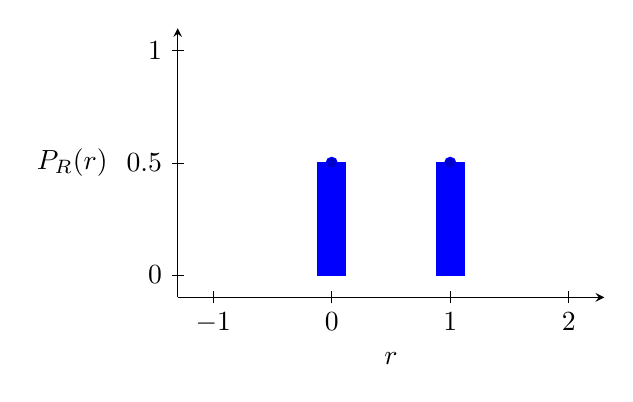
\begin{tikzpicture}
\begin{axis}[
    ymin=0, ymax=1,
    xmin=-1, xmax=2,
    xtick={-1,0,1,2},
    ytick={0,0.5,1},
    axis lines=left,
    width=7cm,
    height=5cm,
    enlargelimits=0.1,
    ylabel={$P_R(r)$},
    xlabel={$r$},
    y label style={rotate=-90}, % match the style in your image
    tick style={black},
    ymajorgrids=false,
    xmajorgrids=false,
    every axis plot/.append style={ybar, bar width=10pt, black, fill=black}
]
\addplot coordinates {(0,0.5) (1,0.5)};
\end{axis}
\end{tikzpicture}
\end{center}

\[
F_R(r) =
\begin{cases}
0 & r < 0, \\
\frac{1}{2} & 0 \le r < 1, \\
1 & r \ge 1 \\
\end{cases}
\]


\begin{center}
\begin{tikzpicture}
\begin{axis}[
    ymin=0, ymax=1.1,
    xmin=-1, xmax=2,
    xtick={-1,0,1,2},
    ytick={0,0.5,1},
    axis lines=left,
    width=7cm,
    height=5cm,
    enlargelimits=0.05,
    xlabel={$r$},
    ylabel={$F_R(r)$},
    y label style={rotate=-90},
    tick style={black},
    every axis plot/.append style={blue, thick},
]

% Use 'const left' for stair-step effect
\addplot[const left] coordinates {
    (-1, 0)
    (0, 0)
    (0, 0.5)
    (1, 0.5)
    (1, 1)
    (2, 1)
};

\end{axis}
\end{tikzpicture}
\end{center}

\end{document}
